\documentclass[12pt]{article}
\usepackage[margin=1.5cm]{geometry}
\usepackage{parskip}
\usepackage{amsmath}
\usepackage{amssymb}
\usepackage{amsfonts}
\usepackage{enumitem}
\usepackage{graphicx}
\usepackage{stmaryrd}
\graphicspath{ {./images/} }


\begin{document}
\begin{enumerate}[label=(\alph*)]
  \item

    We construct the following dynamic programming matrix:

    \begin{tabular}{c|c|c|c|c|c|c|c}
      &$\varepsilon$&C&G&T&G&A&A\\
      \hline
      $\varepsilon$&0&-4&-8&-12&-16&-20&-24\\
      \hline
      G&-4& -3& 1& -3&-7 &-11&-15\\
      \hline
      A&-8& -7&-3&-2 &-6 &-2 &-6\\
      \hline
      C&-12&-3&-7&-6&-5  &-6 &-5 \\
      \hline
      T&-16&-7&-6&-2&-6  &-8 &-9 \\
      \hline
      T&-20&-11&-10&-1&-5&-9 &-11 \\
      \hline
      A&-24&-15&-14&-5&-4&0&-4 \\
      \hline
      C&-28&-19&-18&-9&-8&-4&-3 \\
    \end{tabular}

    Reading backwards from this table, we get the following alignment:

\begin{verbatim}
CG--TGAA
-GAATTAC
\end{verbatim}
        
This is only one of many possible alignments, it should be noted.

\item
  If the sequences have very different lengths, then we would want to choose a small gap penalty, or else sequences with different lengths would be considered inherently dissimilar, but we might want to capture similarities within the sequences themselves, which choosing a smaller gap penalty would help to do.

  Similarly, if we have different base compositions, we may also want a small gap penalty in order to detect well-aligned portions amongst the very different base occurrences.

\item
  The BWT is a transform designed to turn text data into data more suitable for RLE compression, whilst being reversible, essentially improving the performance of RLE compression on data.

  It works by building a matrix of all rotations of a text, sorting them lexicographically, and then outputting the last column:

\begin{verbatim}
GATTACA$
$GATTACA
A$GATTAC
CA$GATTA
ACA$GATT
TACA$GAT
TTACA$GA
ATTACA$G
\end{verbatim}

Then sorting them (treating \$ as lexicographically small), we get:

\begin{verbatim}
$GATTACA
A$GATTAC
ACA$GATT
ATTACA$G
CA$GATTA
GATTACA$
TACA$GAT
TTACA$GA
\end{verbatim}

Then taking the last column, we get \texttt{ACTGA\$TA} as the BWT.

To reverse this, we realise that we can generate all successive pairs of characters by sorting the BWT, generating the first column:

\begin{verbatim}
$ A
A C
A T
A G
C A
G $
T T
T A
\end{verbatim}

So by reading from the EOF character to the corresponding character in the first column (G), we know that the string just begin with \texttt{G}. By repeating this process (looking across from G to see A, and specifically the third A), we know the text must read \texttt{GA}. By repeating this process, we can reconstruct the original text.

\item
  In this context, biologists may have gathered the expression of every gene in a particular organism over a time period (and perhaps varying conditions). By treating the expression of a gene over $n$ time points as an $n$-dimensional vector, we can find similar behaving genes (those that express at similar times), by clustering these $n$-dimensional vectors in space.

  This clustering can be done in many ways, but the general idea is to separate the points (or genes) into sets, where each set contains similar points. A good clustering should ensure that all points in a particular cluster are closer to each other than they are to points in different clusters.

  Many techniques exist to find clusters. For example, if we know how many clusters we wish to generate, say $k$, we can generate $k$ centers, and assign each point its closest center. Then, we gradually adjust each center closest to the center of its assigned points. Iterating this process generates clusters.

  If we do not know how many clusters we want, we can use something like UPGMA, which generates a hierarchy of clusters, which we can cut off at any point.

\item
  The UPGMA algorithm works by assigning each element a unique cluster, and then progressively joining clusters together based on the average distance between elements in each cluster.

  For example, when we apply UPGMA to the given distance matrix, we get the following tree, representing each cluster:

  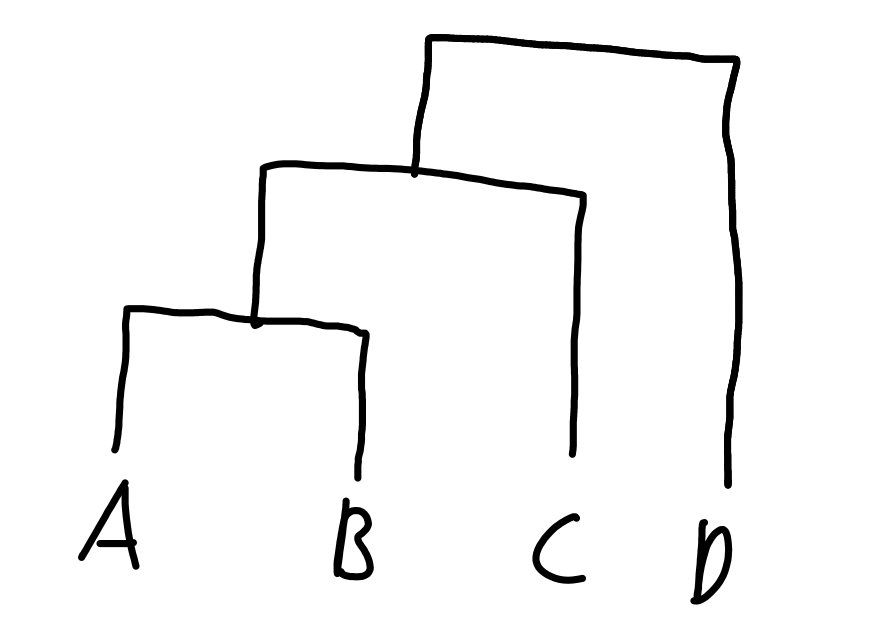
\includegraphics[scale=0.3]{upgma}


\end{enumerate}
\end{document}
